% Specification of length of, and dates for, first iteration.

Our first iteration started on 22/10/10 and will end after two weeks on 05/11/10.
In the beginning of the iteration all team members acquired a theoretical understanding
of the task by reading journal articles on description logic and proof/model searching.
We decided to use Haskell as programming language language and agreed on a general
design (see Figure~\ref{design}). The tasks for our first iteration are derived from
this design; they are listed in the sprint backlog in Table~\ref{sprint}.

\begin{figure}
  \caption{The general design of the program.}
  \begin{center}
    \includegraphics[scale=0.4]{design.jpeg}
  \end{center}
  \label{design}
\end{figure}

% Details mapping of iteration tasks onto group members (-> Sprint backlog).

\begin{table}
  \caption{Sprint backlog.}
  \begin{tabular}{l|l|l}
    %\hline
    %\multicolumn{2}{|c|}{Tasks} \\
    \hline
    \textbf{Task} & \textbf{Owner} & \textbf{To be completed by} \\
    \hline
    specification of concept as Haskell data type & group & 29/10/10 \\
    specification of model as Haskell data type & group & 29/10/10 \\
    specification of proof as Haskell data type & group & 29/10/10 \\
    implementation of proof/model search for $\mathcal{AL}$ & Jannis, Saguy & 29/10/10 \\
    implementation of model checker for $\mathcal{AL}$ & Michal & 05/11/10 \\
    implementation of proof checker for $\mathcal{AL}$ & Ka Wai & 05/11/10
  \end{tabular}
  \label{sprint}
\end{table}

% Identification of potential risks during first iteration.

In order to successfully complete the first iteration everyone needs to have a good
understanding of the underlying theory. We need to identify suitable algorithms and
adapt them to our setup. 

There is a risk that we will spend more time on theory than expected, but we will keep
track of this in our regular meetings and adapt our time plan if necessary.
Another possible risk is that our chosen blend
of development method does not work as intended; we will regularly reflect on this as well
and possibly drop parts that are not helping us. A final risk is we may not be able
to find implementations that run in feasible time, but from our first explorative reading
we are confident that we will be able to handle that risk, possibly improving performance
in later iterations.


To minimise this risk, we aim to implement the most basic functionality first while
still producing a complete working program in the first iteration. The design will
allow extending this functionality in further iterations.

We will spend much time on design and theory to provide a design that can be extended
in later iterations. The remainder will be spent on implementation and testing.

% Planned progress measure for first iteration.

Our objective for the first iteration is a fully working program that, given an
$\mathcal{AL}$ concept, produces either a model for that concept or a proof showing its
unsatisfiability. Both proof and model can be checked for correctness by the program.

The progress to achieve this goal is measured by regular meetings (twice a week) where
we will discuss the progress so far, identify problems and determine the next tasks. This
way we will always exactly know how far we are from completing the iteration.

